\documentclass[tikz]{standalone}

\usepackage{tikz}
\usetikzlibrary{trees}
\usetikzlibrary{shapes}
\usetikzlibrary{positioning}
\usetikzlibrary{arrows.meta}

\tikzset{
    pointer/.style = {thick,draw=black,triangle 45-*,shorten >=-3pt},
    cell/.style = {rectangle, thick, draw=black,minimum width = 1cm, minimum height =1.0cm,fill=yellow!20},
    mynode/.style = {circle, thick, draw=black, align=center,fill=yellow!40,font=\ttfamily\bfseries\Large},
    mynoder/.style = {circle, thick, draw=black, align=center,fill=red!30,font=\ttfamily\bfseries\Large},
    mynodeb/.style = {circle, thick, draw=black, align=center,fill=blue!30,font=\ttfamily\bfseries\Large},
    edgen/.style = {-latex,ultra thick},
    edger/.style = {-latex,ultra thick,red},
    edgeb/.style = {-latex,ultra thick,blue},
    edgeg/.style = {-latex,ultra thick,gray},
    edgegd/.style = {-latex,ultra thick,brown,dashed}, % back
    edgevd/.style = {-latex,ultra thick,violet,dotted}, % forward
    edgexd/.style = {-latex,ultra thick,blue,densely dotted}, % traversal
    every picture/.style={/utils/exec={\ttfamily\bfseries}},
    every picture/.style={font issue=\ttfamily\bfseries},
    font issue/.style={execute at begin picture={#1\selectfont}
  }
}

\newcommand{\R}[1]{\textcolor{red}{#1}}
\newcommand{\B}[1]{\textcolor{blue}{#1}}
\newcommand{\G}[1]{\textcolor{violet}{#1}}

\begin{document}

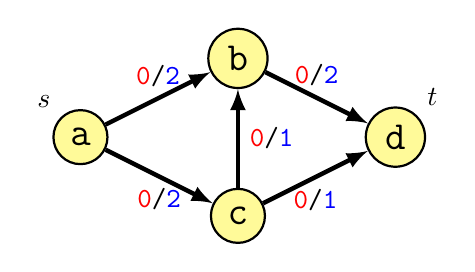
\begin{tikzpicture}[scale=1.00,transform shape]
\node[mynode, label={above left:$s$}] at (0.0, 1.0) (a) {a};
\node[mynode] at (2.0, 2.0) (b) {b};
\node[mynode] at (2.0, 0.0) (c) {c};
\node[mynode, label={above right:$t$}] at (4.0, 1.0) (d) {d};
\draw[edgen] (a) edge[above] node {\R{0}/\B{2}} (b);
\draw[edgen] (a) edge[below] node {\R{0}/\B{2}} (c);
\draw[edgen] (c) edge[right] node {\R{0}/\B{1}} (b);
\draw[edgen] (c) edge[below] node {\R{0}/\B{1}} (d);
\draw[edgen] (b) edge[above] node {\R{0}/\B{2}} (d);
\end{tikzpicture}


\end{document}